\documentclass[a4paper,12pt]{article}
\usepackage[utf8]{inputenc}
\usepackage[english]{babel}
\usepackage{fancyhdr}
%Use this to customize margins
\usepackage[
  top=2cm,
  bottom=2cm,
  left=1cm,
  right=1cm,
  headheight=17pt, % as per the warning by fancyhdr
  includehead,includefoot,
  heightrounded, % to avoid spurious underfull messages
]{geometry} 

%Use this to customize headers
\pagestyle{fancy}
\fancyhf{}
\fancyhead[LE,RO]{Report version: \today}
\fancyhead[RE,LO]{ReMeltRadar 2021/22}
\fancyfoot[CE,CO]{\leftmark}
\fancyfoot[LE,RO]{\thepage}
\usepackage{graphicx}
\renewcommand{\headrulewidth}{2pt}
\renewcommand{\footrulewidth}{1pt}


\usepackage{blindtext}

%Use this to customize tables
\usepackage[table]{xcolor}
\setlength{\arrayrulewidth}{1mm}
\setlength{\tabcolsep}{18pt}
\renewcommand{\arraystretch}{1.5}
\linespread{1.25} % also use linespacing > 1? JH 2022-03-21
%\arrayrulecolor[HTML]{fffff}

%Use this to customize colors
\definecolor{babyblueeyes}{rgb}{0.63, 0.79, 0.95}
\definecolor{beaublue}{rgb}{0.74, 0.83, 0.9}
\definecolor{bluegray}{rgb}{0.4, 0.6, 0.8}

%Here some pre-defined commands
\newcommand{\ProtocolTable}[6]
{
\begin{table}[]
\begin{tabular}{|p{1.8cm} p{3.8cm} p{1.8cm} p{2.0cm}|}
\hline
 \rowcolor{beaublue}\textbf{Name}:&\multicolumn{3}{l}{#1} \\
 \rowcolor{beaublue}\textbf{Folder:}&\multicolumn{3}{l}{#2} \\
 \rowcolor{beaublue}\textbf{Instrument:}&#3&\textbf{Date:}&#4 \\
  \rowcolor{beaublue}\textbf{Operator:}&#5&\textbf{Location:}&#6\\
\hline
\end{tabular}
\end{table}
}

% JH Added Packages
\usepackage[bottom]{footmisc}
\usepackage{siunitx}
\usepackage[outline]{contour}
\usepackage{tikz}
\usetikzlibrary{positioning,calc}
\usepackage{circuitikz}

\definecolor{ucl_red}{HTML}{D50032}
\definecolor{UCLdarkblue}{HTML}{003D4C}

% Define ApRESDOC command to show details of ApRES profiles
\newcommand{\apresdoc}[9]{
    \def\tempapfname{#1}
    \def\tempaploc{#2}
    \def\tempapcom{#3}
    \def\temptimestamp{#4}
    \def\tempafgain{#5}
    \def\temprfattn{#6}
    \def\tempperiod{#7}
    \def\tempflow{#8}
    \def\tempfupp{#9}
    \apresdoccont
}
\newcommand{\apresdoccont}[6]{
  \def\tempnatt{#1}
  \def\tempnchirp{#2}
  \def\tempnsubburst{#3}
  \def\temppowercode{#4}
  \def\tempbattvolt{#5}
  \def\tempaplbl{#6}

  \begin{table}
    \caption{\tempapcom}
    \rowcolors{2}{gray!25}{white}
    \centering
    \includegraphics[width=0.9\textwidth]{Figures/ApRES/Rover/HF/\tempapfname.png}
    \\
    ~\\
    \begin{tabular}{>{\bfseries}l l >{\bfseries}l l}
      \hline
      \rowcolor{gray!50}
      \multicolumn{4}{c}{\textbf{Filename} \tempapfname} \\
      \hline
      Param. & \bfseries Value & Param. & \bfseries Value \\
      AF Gain & \tempafgain &
      RF Attn. & \temprfattn \\
      Subbursts & \tempnsubburst &
      Period ($T$) & \tempperiod~s \\
      Bandwidth & \tempflow~-~\tempfupp~MHz &
      Power Code & \temppowercode \\
      Batt. Volt. & \tempbattvolt~V &
      - & - \\
      \hline
    \end{tabular}
    \label{\tempaplbl}
  \end{table}
}

%Start the document here.

\begin{document}
\section{Summary of ReMeltRadar 2021/22}
\textbf{RD}

\begin{figure}
  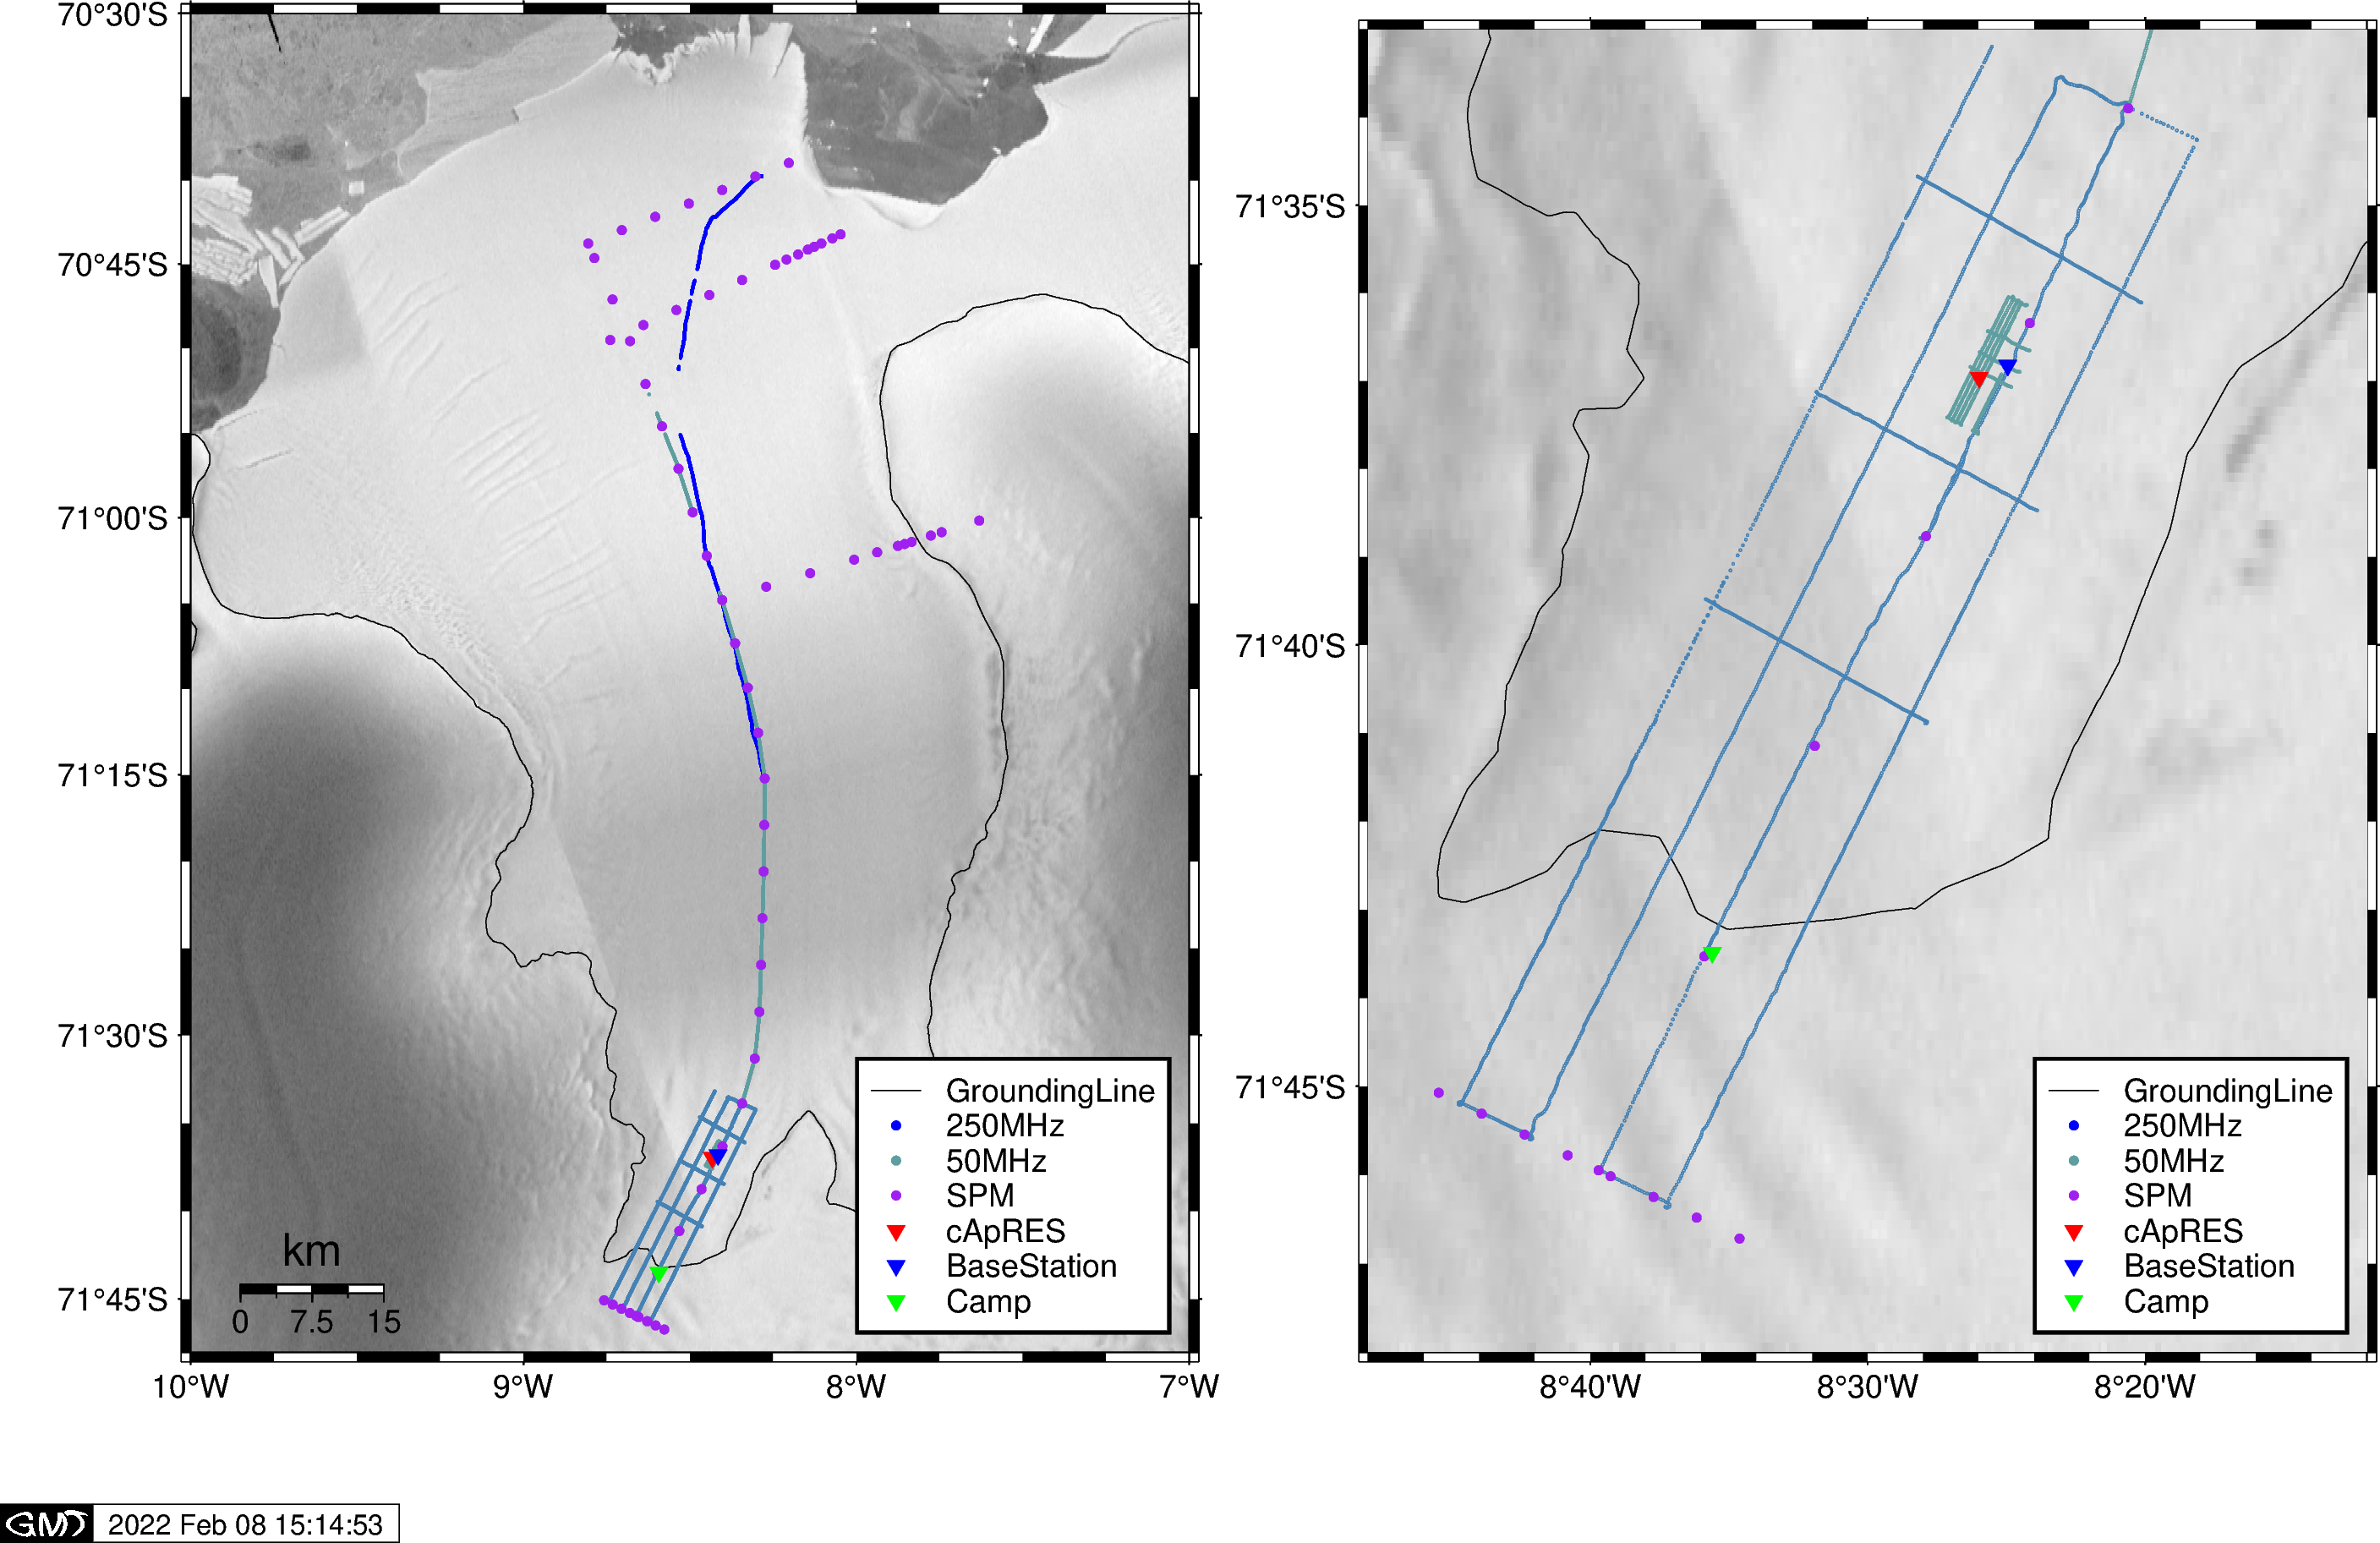
\includegraphics[width=\linewidth]{Figures/Overview.png}
  \caption{(Left) Larger-scale bird's eyes perspective of 250 MHz GPR, 50 MHz GPR, static \& polarimetric (SPM) and continuous ApRES (cApRES) locations at Ekström Ice Shelf, East Antarctica. (Right) Close-up of the survey grid close to the grounding-zone.}
  \label{fig:overview}
\end{figure}
ReMeltRadar's scientific focus (1) to understand \& quantify processes that govern ocean-induced melting at the base of ice shelves, and (2) to provide observational constraints on the spatial variability of ice rheology impacting ice-shelf buttressing strength. The area of interest is the Ekström Ice Shelf, East Antarctica, using the Neuyamer III station as a logistical hub for field surveys on the ice shelf and in the grounding zone. The first field season took place from November 2021 to January 2022. This report details the data collected and will serve as a baseline for envisaged repeat measurements in 2022/23. 

\pagebreak
\subsection{Team composition and chronology of data collection}
\begin{table}
\rowcolors{2}{gray!25}{white}
\begin{tabular}{llll}
  \rowcolor{gray!50}
  Name & Project& Deployment& Responsibility\\
  \hline
  Inka Koch (UT) & ReMeltRadar & 27.12.21-13.12.22& PulseEkko GPR\\
  Jonathan Hawkins (UCL) & ReMeltRadar  &27.12.21-13.12.22& HF ApRES\\
  Reinhard Drews (UT) & ReMeltRadar  &27.12.21-13.12.22& Science Coordination\\
  Reza Ershadi (UT) & ReMeltRadar &05.11.21-13.12.22& Rover, SPM\\
  Olaf Eisen (AWI) & ReMeltRadar  &05.11.21-13.12.22& Traverse Leader\\
  \hline
\end{tabular}
\caption{\label{TableGPR}Team composition of ReMeltRadar with members of University of Tübingen (UT), University College London (UCL), and Alfred Wegener Institute (AWI).}
\end{table}
\begin{table}
  \rowcolors{2}{gray!25}{white}
  \begin{tabular}{m{1.5cm} m{2.25cm} m{7cm} m{3cm}}
    \rowcolor{gray!50}
    Date & Frequency & Profile & File-ID\\
    \hline
    28.12.21 & 50, 100 MHz & Test profiles near NM& \textit{PE files}\\
    29.12.21 & 100 MHz & MPA01-MPA03, SPX4-SPX2 near NM& \textit{PE files}\\
    01.01.22 & 250 MHz  & NM-SPMA25 during traverse& \textit{PE files}\\
    02.01.22 & 50 MHz & GZ profiling along flow (SPMA25-SPMA21-GLPE3n-GLPE4s)& \textit{PE files}\\
    03.01.22 & 50 MHz & GZ profiling along flow (GLPE4s-GLPE1s-GLPE2n transfer to SPMA25)& \textit{PE files}\\
    04.01.22 & 50 MHz & GZ profiling along flow (GLPE7n-GLPE8s-GLPE5s)& \textit{PE files}\\
    05.01.22 & 50 MHz & GZ profiling across flow (XX points XX)& \textit{PE files}\\
    06.01.22 & 50 MHz & Finegrid along flow (XX points XX)& \textit{PE files}\\
    09.01.22 & 50 MHz & Finegrid across flow (XX points XX)& \textit{PE files}\\
    10.01.22 & 50 MHz & Along-flow Camp-NM (SPMA21-SPMA10)& \textit{PE files}\\
    12.01.22 & 50 MHz & Camp-NM continuation (SPMA10 - XX)& \textit{PE files}\\
    \hline
  \end{tabular}
  \caption{\label{TableGPR}Overview of GPR measurements taken with the PulseEkko radar from Sensors\&Software. Details for the system setup and individual profiles are found in Section \ref{SecGpr}. Operator: I. Koch.}
Here we need a table such as table \label{TableGPR} for each sensor. 
\end{table}

\pagebreak
\section{Data structure and initial source codes}
\textbf{RD, JH}

\pagebreak
\section{GPR: Data example, field picture, system setup and profile specifics}
\label{SecGpr}
\textbf{IK}
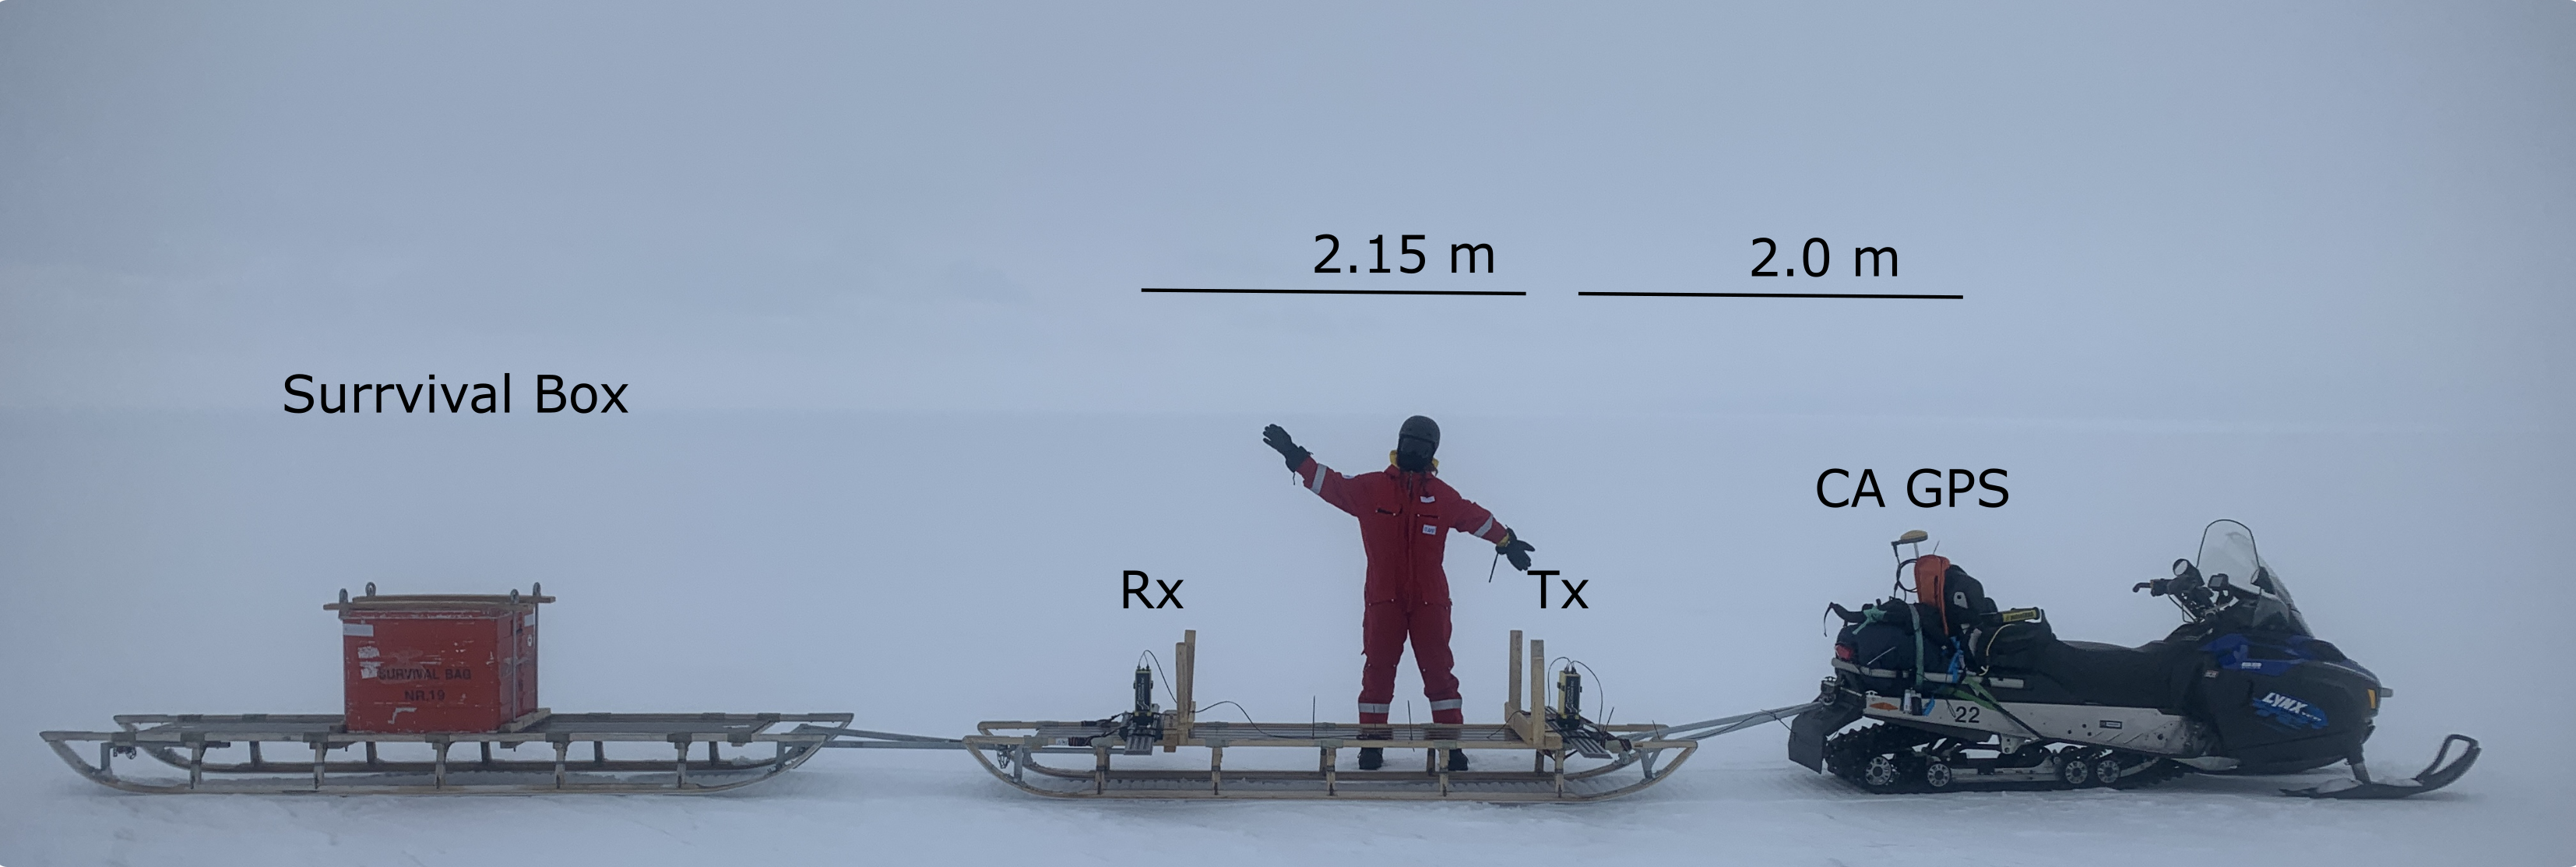
\includegraphics[width=\textwidth]{Figures/PulseEkko/RadarSetup.png}

\pagebreak
\section{SPM: Data example, field picture, system setup and site specifics}
\textbf{RE}
\label{SecSPM}

\pagebreak
\section{HF ApRES}
%: Data example, field picture, system setup and profile specifics
\label{SecHFApRES}

\subsection{System Overview}
The HF ApRES is a frequency modulated continuous wave (FMCW) radar operating
over a bandwidth of \SI{20}{\mega\hertz} to \SI{40}{\mega\hertz}.  It builds
upon the existing phase-coherent radar architecture of the ApRES\footnote{
  P. Brennan, L. Lok, K. Nicholls and H. Corr, "Phase‐sensitive FMCW radar 
  system for high‐precision Antarctic ice shelf profile monitoring", IET 
  Radar, Sonar \& Navigation, vol. 8, no. 7, pp. 776-786, 2014. Available: 
  10.1049/iet-rsn.2013.0053.
} but uses a modified radio front-end to operate at the reduced bandwidth
described.  In addition to the radar, the HF ApRES makes use of two 'wire-mesh
dipole' antennas - one each for the transmitter and receiver, and a 12V 
\SI{7}{\ampere\hour} lead-acid battery for power.  Testing was required 
to validate the performance of both the HF ApRES radar unit and 
'wire-mesh dipole' antennas, as they had not been previously deployed on a 
polar ice shelf and subject only to verification through simulation and 
laboratory testing.

\subsubsection{System Equipment Listing}
\begin{itemize}
  \item 1x HF ApRES (VAB Issue C and RMB2F in Pelicase)
  \item 2x Wire-Mesh Dipole Antennas
  \item Clusons 12V \SI{7}{\ampere\hour} Lead Acid Battery
  \item 4x Radiall RG213 \SI{5}{\metre} 50$\Omega$ RF Cables (R284C0351044)
  \item 2x Gigatronix LBC400 \SI{25}{\metre} 50$\Omega$ RF Cables (APX2KDP6ZAB40L)
  \item 2x \SI{10}{\deci\bel} RF attenuators
  \item Various RF connectors
  \item Bamboo and 10mm kernmantle rope for towed configuration.
\end{itemize}

\begin{figure}[htbp]
  \centering
  
  \begin{tikzpicture}[font=\sffamily]
    \node[above right, inner sep=0, draw, black, line width=2pt] (img) at (0,0) {
      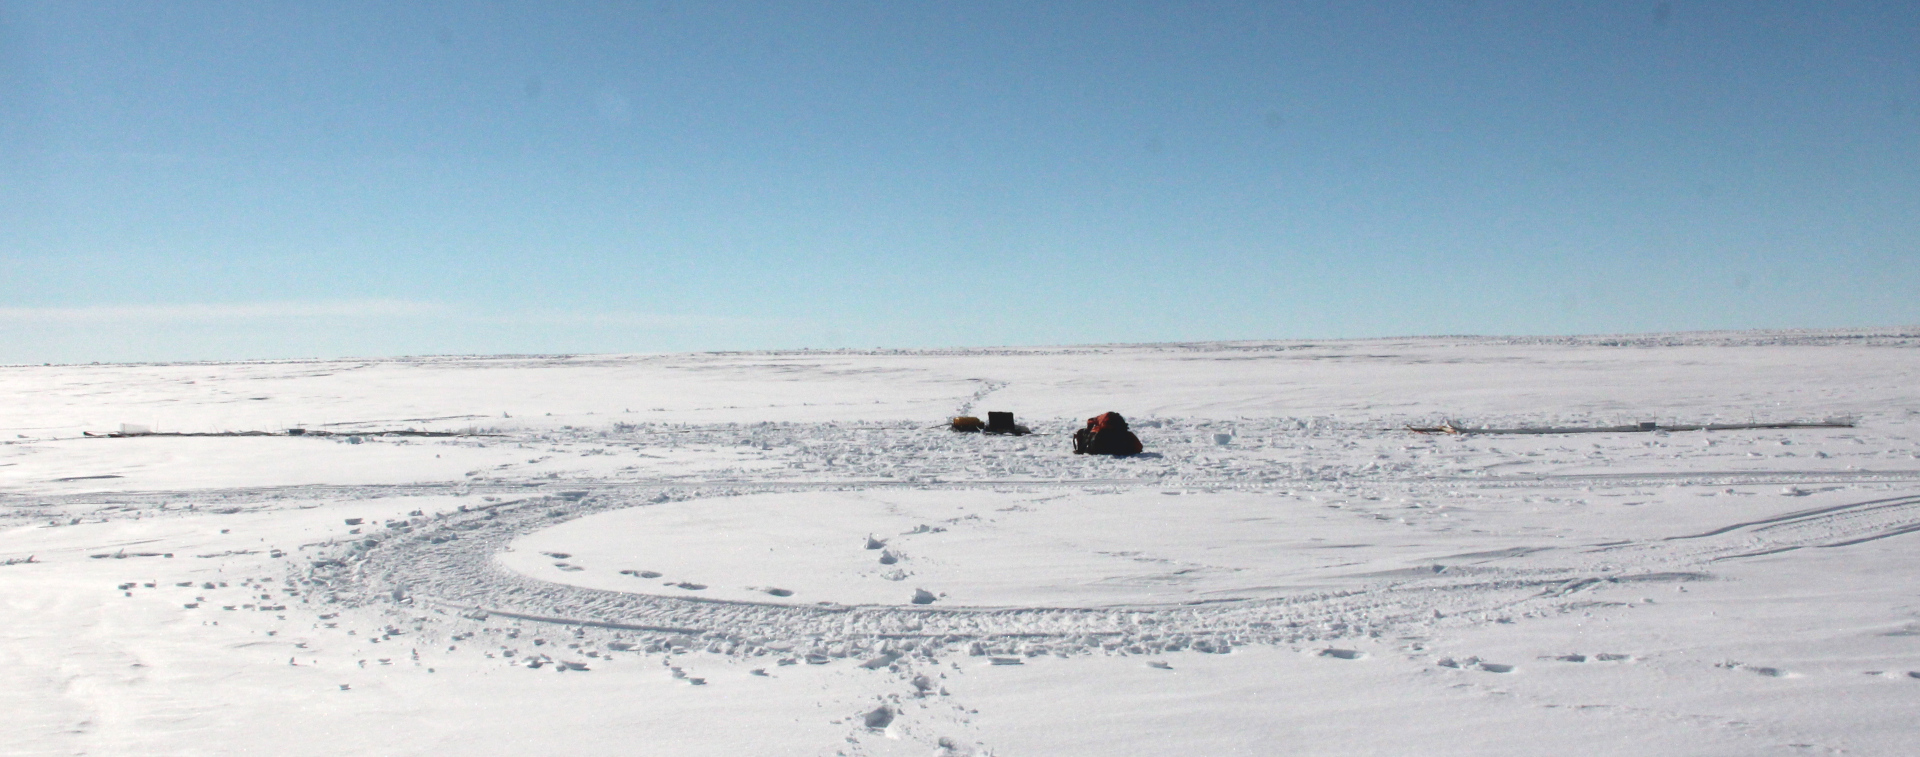
\includegraphics[width=0.9\textwidth]{Figures/ApRES/Rover/HF/hf-apres-neumayer.jpg}
    };
    \begin{scope}[x={(img.south east)}, y={(img.north west)}]
      
      % Temporary grid
      % \draw[gray,step=0.1] (img.south west) grid (img.north east);
      % End temporary grid
      \contourlength{1pt}
      \node (tx_ant) at (0.16,0.375) {\contour{white}{\bfseries Tx Antenna}};
      \node (rx_ant) at (0.85,0.375) {\contour{white}{\bfseries Rx Antenna}};
      \node (rx_ant) at (0.5,0.5) {\contour{white}{\bfseries HF ApRES}};

      \draw[latex-latex,ucl_red,line width=1pt] (0.25,0.38) -- 
      node[midway,below] {\contour{white}{\bfseries 5-15m (End-End)}} (0.73,0.38);

      \draw[latex-latex,ucl_red,line width=1pt] (0.16,0.6) -- 
      node[midway,above] {\contour{white}{\bfseries 10-20m (Phase Centres)}} (0.85,0.6);
    
    \end{scope}

  \end{tikzpicture}


  \caption{
    Deployed HF ApRES radar positioned in centre of transmit (Tx) and receive
    (Rx) antennas in endfire configuration.
  }
  \label{FigHFApRESNeumayer}
\end{figure}

\subsection{Testing Summary}
Testing was first conducted with the wire-mesh antennas to verify that they 
met the power transfer characteristics predicted through simulation.  Once
verified, a setup with the full HF ApRES system was configured and issues
were found with strong coupling between the transmit and receive antennas.
After further testing, it was found that broadside orientation of the antennas
and increased separation reduced the direct coupling between the antennas 
sufficiently for clean deramped signals to be recorded.


\begin{table}
  \rowcolors{2}{gray!25}{white}
  \begin{tabular}{m{1.5cm} m{2.25cm} m{7cm} >{\raggedright\arraybackslash}m{3cm}}
    \rowcolor{gray!50}
    Date & Frequency & Profile & File-ID\\
    \hline
    27.12.21 & 30 MHz & Testing of antennas and HF ApRES near Neumayer & \textit{Testing.db} \\
    28.12.21 & 30 MHz & (as above) & \textit{Testing.db} \\
    29.12.21 & 30 MHz & (as above) & \textit{Testing.db} \\
    30.12.21 & 30 MHz & (as above) & \textit{Testing.db} \\
    02.01.22 & 30 MHz & Testing of HF ApRES at Camp & \textit{Testing.db} \\
    03.01.22 & 30 MHz & (as above) & \textit{Testing.db} \\
    04.01.22 & 30 MHz & (as above) & \textit{Testing.db} \\
    05.01.22 & 30 MHz & (as above) & \textit{Testing.db} \\
    06.01.22 & 30 MHz & Testing of HF ApRES at Camp and relocate to GL & \textit{Testing.db} \\
    07.01.22 & 30 MHz & Initial measurements of start-stop survey at GL & \textit{Testing.db, StartStop.db} \\
    08.01.22 & 30 MHz & Complete measurement of start-stop survey at GL and attempt kinematic surveys & \textit{Testing.db, StartStop.db} \\
    \hline
  \end{tabular}
  \label{TableHFApRES}
  \caption{Overview of measurements taken with HF ApRES System} 
\end{table}

\subsubsection*{Wire-Mesh Dipole Antennas}
The wire-mesh dipole antennas were each tested with an SDRKits Vector Network
Analyzer (VNA) which allows for the measurement of the antenna reflection
coefficient ($\Gamma$).  The reflection coefficient is calculated from the
scattering parameters (s-parameters) measured by the VNA, where $S_{11}$ 
refers to the phasor ratio between the scattered and incident voltages from
the antenna.  The reflection coefficient can therefore be used to infer the 
ratio of incident power to the antenna which is 'accepted' and sets an upper
bound on the radiation efficiency.  The radiation efficiency of the antenna
is the ratio of incident power to the antenna that is actually radiated
rather than scattered back to the radar, or lost through conduction within the
antenna structure.  Radiation efficiency is difficult to measure in a field 
environment, hence the reflection coefficient is used to determine an upper
bound.

\begin{equation}
  \left|\Gamma\right|_{\texttt{dB}} = 20\log_{10} \left|S_{11}\right|
\end{equation}

The measured reflection coefficient of the wire-mesh dipole antennas from tests
on 28.12.21 is shown in Figure \ref{FigureWireMeshNeumayer}.  Within the field
of antenna engineering, a reflection coefficient of less than
\SI{-10}{\deci\bel} across the desired signal bandwidth, i.e. greater than 90\%
of power accepted by the antenna, is deemed to be acceptable.  It can be seen
that during initial tests conducted \SI{500}{\metre} south-west of Neumayer
Station the antennas have a measured $\left|S_{11}\right|_{\textrm{dB}}$ of less
than \SI{-10}{\deci\bel} across the desired signal bandwidth of
\SI{20}{\mega\hertz} to \SI{40}{\mega\hertz}.  Discussion regarding the antenna
orientation can be found in Section ???.

\paragraph*{Note:} After transport of the antennas from Neumayer III to the
grounding line camp, it was found that one of the centre-pin conductors on the
antenna arms had become loose, likely due to a dry solder joint.

\begin{figure}[htbp]
  \centering
  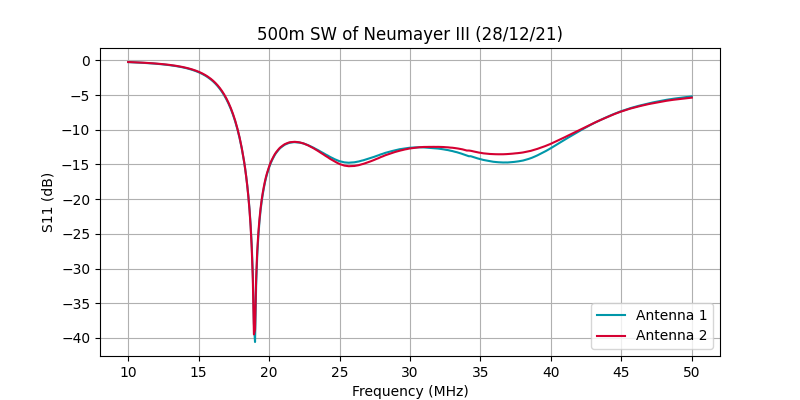
\includegraphics[width=\textwidth]{Figures/ApRES/Rover/HF/antenna_comparison_s11.png}
  \caption{
    Measured power reflection coefficient for HF wire-mesh dipole antennas, 
    positioned approximately \SI{500}{\metre} south-west of Neumayer Station.
  }
  \label{FigureWireMeshNeumayer}
\end{figure}

\subsubsection*{HF ApRES Radar}
Figure \ref{FigureHFApRESNoReceiveAntenna} shows a meaured test profile at
Neumayer Station where it was discovered that the receiving antenna of the HF
ApRES radar was disconnected.  A radar echo from is visible at approximately 
\SI{250}{\metre} depth, which corresponds with the expected thickness of the ice
shefl in the vicinity of the station.  The working explaination for the clear,
high signal-to-noise ratio (SNR) echo from the ice-shelf base with no receiving
antenna is that the echo is received by the transmitting antenna and coupled to
the mixer through the ADP-2-1W power divider to the ADE-1HW mixer, shown in
Figure \ref{FigureHFApRESRadarArchitecture}.

\begin{figure}[h]
  \centering
  \begin{circuitikz}[font=\scriptsize,american,scale=0.75,transform shape,node distance=1.6]

  \coordinate (dds_out) at (0,0);
  \coordinate[right=of dds_out] (dds_attn);
  \coordinate[right=of dds_attn] (adl5535);
  \coordinate[right=of adl5535] (adl5535_attn);
  \coordinate[right=of adl5535_attn] (grf5010);

  \draw (dds_out) to[short,-o] ($ (dds_out) + (-0.1,0) $) node[anchor=east] {DDS Out};

  %\draw (dds_out) to[twoport,t=Attn,l=\SI{9}{\deci\bel}] (dds_attn);
  \draw (dds_out) to[twoport,n=9db,l=\SI{9}{\deci\bel}] (dds_attn);
  %\draw (dds_out) -- ++(0.4,0) -- ++(0.075,0.1) -- ++(0.15,-0.2) -- ++(0.15,0.2) -- ++(0.15,-0.2) -- ++(0.15,0.2) -- ++(0.075,-0.1) -- (dds_attn);
  \coordinate (dds_attn_symb) at ($(dds_out)!0.5!(dds_attn)$);
  \draw (dds_attn_symb) -- ++(0.1,0.075) -- ++(-0.2,0.15) -- ++(0.2,0.15);
  \draw (dds_attn_symb) -- ++(-0.1,-0.075) -- ++(0.2,-0.15) -- ++(-0.2,-0.15);

  \draw (dds_attn) to[amp,l=ADL5535] (adl5535);

  %\draw (adl5535) to[twoport,t=Attn,l=\SI{12.2}{\deci\bel}] (adl5535_attn);
  \draw (adl5535) to[twoport,l=\SI{12.2}{\deci\bel}] (adl5535_attn);  
  %\draw (adl5535) -- ++(0.4,0) -- ++(0.075,0.1) -- ++(0.15,-0.2) -- ++(0.15,0.2) -- ++(0.15,-0.2) -- ++(0.15,0.2) -- ++(0.075,-0.1) -- (adl5535_attn);
  \coordinate (tx_attn_symb) at ($(adl5535)!0.5!(adl5535_attn)$);
  \draw (tx_attn_symb) -- ++(0.1,0.075) -- ++(-0.2,0.15) -- ++(0.2,0.15);
  \draw (tx_attn_symb) -- ++(-0.1,-0.075) -- ++(0.2,-0.15) -- ++(-0.2,-0.15);

  \draw (adl5535_attn) to[amp,l=GRF5010] (grf5010);

  \node[wilkinson] at ($ (grf5010) + (1, 0) $) (power_divider) {ADP-2-1W};

  \draw (power_divider.out2) to[short,-o] ($ (power_divider.out2) + (0.5,0) $) node[anchor=west] (rf_out) {TX Out};
  \draw (power_divider.out1) to[short] ($ (power_divider.out1) + (0.5,0) $) node (mix_out) {};

  \coordinate[below=of power_divider.out1] (mix_bpf);
  \coordinate[left=of mix_bpf] (mix_attn);
  \coordinate[left=of mix_attn] (rf_out_mix);

  \draw (mix_out.center) |- (mix_bpf);
  \draw (mix_bpf) to[bandpass,l_=JCBP-43+] (mix_attn);
  %\draw (mix_attn) to[twoport,t=Attn,l_=\SI{2.5}{\decibel}] (rf_out_mix);
  \draw (mix_attn) to[twoport,l_=\SI{2.5}{\decibel}] (rf_out_mix);
  %\draw (rf_out_mix) -- ++(0.4,0) -- ++(0.075,0.1) -- ++(0.15,-0.2) -- ++(0.15,0.2) -- ++(0.15,-0.2) -- ++(0.15,0.2) -- ++(0.075,-0.1) -- (mix_attn);
  \coordinate (mix_attn_symb) at ($(rf_out_mix)!0.5!(mix_attn)$);
  \draw (mix_attn_symb) -- ++(0.1,0.075) -- ++(-0.2,0.15) -- ++(0.2,0.15);
  \draw (mix_attn_symb) -- ++(-0.1,-0.075) -- ++(0.2,-0.15) -- ++(-0.2,-0.15);

  \coordinate[below=1.75cm of rf_out_mix] (below_rf_out);

  \coordinate (deramp_in) at (dds_out |- below_rf_out);
  \draw (deramp_in) to[short,-o] ($ (deramp_in) + (-0.1,0) $) node[anchor=east,align=left] {Deramp\\Filter In};
  
  \node[mixer,right=0.25cm of deramp_in] (mix) {};
  \draw (deramp_in) -- (mix.1);
  \draw[latex-] (mix.4) |- (rf_out_mix);

  % Create cross-point coordinate with DDS output and in-line with mixer
  \coordinate (rf_in) at (power_divider.out2 |- mix.3);
  \draw (rf_in) to[short,-o] (rf_in -| mix_out) node[anchor=west] {RX In};

  \coordinate[left=of rf_in] (rf_in_bpf);
  \coordinate[left=1.3cm of rf_in_bpf] (lna1);
  \coordinate[left=1.3cm of lna1] (dsa);
  \coordinate[left=1.3cm of dsa] (lna2);

  % Start RF Input chain
  \draw (rf_in) to[bandpass,l=JCBP-43+] (rf_in_bpf);
  \draw (rf_in_bpf) to[amp,l_=LHA-13LN+] (lna1);
  \draw (lna1) to[twoport,t=\scriptsize DSA,l=F1958] (dsa);
  \draw (dsa) to[amp,l_=LHA-13LN+] (lna2);
  %\draw (lna2) to[twoport,t=Attn,l=\SI{9}{\deci\bel}] (mix.3);
  \draw[-latex] (lna2) to[twoport,l=\SI{9}{\deci\bel}] (mix.3);
  %\draw (mix.3) -- ++(0.4,0) -- ++(0.075,0.1) -- ++(0.15,-0.2) -- ++(0.15,0.2) -- ++(0.15,-0.2) -- ++(0.15,0.2) -- ++(0.075,-0.1) -- (lna2);
  \coordinate (rx_attn_symb) at ($(mix.3)!0.5!(lna2)$);
  \draw (rx_attn_symb) -- ++(0.1,0.075) -- ++(-0.2,0.15) -- ++(0.2,0.15);
  \draw (rx_attn_symb) -- ++(-0.1,-0.075) -- ++(0.2,-0.15) -- ++(-0.2,-0.15);

  \node[anchor=north] at ($ (mix.2) + (0,-0.05) $) {ADE-1HW};
  
\end{circuitikz}

  \caption{
    System level diagram of the RMB2F radar, showing the signal path from the
    direct digital synthetiser (DDS) to the transmit output, receiver input and
    ouput deramped FMCW signal.}
  \label{FigureHFApRESRadarArchitecture}
\end{figure}

\apresdoc
{2021-12-28\_213752.dat}
{Neumayer III}
{Antennas aligned E-W, no receive antenna connected but clear return from
ice-shelf base and double bounce.}
{2021-12-28 21:37:53.000}
{6,6,6,6}
{30,20,10,0}
{1.000}
{20}
{40}
{4}
{40}
{10}
{127}
{12.129}
{FigureHFApRESNoReceiveAntenna}

Reconnecting the receiver antenna, as shown in Figure
\ref{FigureHFApRESReconnectedAntenna} results in sigificant distortion visible
in the time-domain FMCW voltage signal, matched with the reduced SNR seen in the
range-power profile.  Overall power is increased relative to Figure
\ref{FigureHFApRESNoReceiveAntenna}, which gives confidence that the antenna was
not connected and has been successfully reconnected in the second dataset.  The
distortion is characteristic of 'clipping' where the recorded signal exceeds the
voltage range of the analogue-to-digital converter and the output is
subsequently 'clipped' to be within this range.  The evidence of clipping, at
low frequencies corresponding to short range echoes suggests that the direct
coulping between the antennas is higher than experienced from a previous
deployment of the HF ApRES radar on an Alpine glacier. 

\apresdoc
{2021-12-28\_214326.dat}
{Neumayer III}
{Antennas aligned E-W, receive antenna reconnected and low-frequency (i.e. near
range) distortion present in signal resulting in reduced signal-to-noise ratio.}
{2021-12-28 21:43:26.000}
{6,6,6,6}
{30,20,10,0}
{1.000}
{20}
{40}
{4}
{40}
{10}
{127}
{12.158}
{FigureHFApRESReconnectedAntenna}

\paragraph*{Antenna orientation} was shown to be related to the coupling between
the transmit and receive antennas and the presence of high-power low frequency
signals in the deramped FMCW voltage signal.  Broadside refers to the antennas
positioned such that their phase centres are in line with the survey direction
and their longest axes are orthogonal to the survey direction.  Endfire refers
to the antennas positioned such that their longest axes are parallel to the
survey direction.  Experiemnts repeated at Neumayer Station and the grounding
line camp show that thwne antennas are aligned in a 'broadside' configuration
they exhibit reduced near-range coupling compared to antennas separated by the
same distance in an 'endfire' configuration.  The HF ApRES was then reconfigured to be operated with the SubZero rover in a
broadside configuration, with an increased separation between the
transmit and receive antennas of \SI{40}{\metre}.

\begin{figure}[htbp]
  \centering
  \begin{tikzpicture}[font=\sffamily]
    \node[above right, inner sep=0, draw, black, line width=2pt] (img) at (0,0) {
      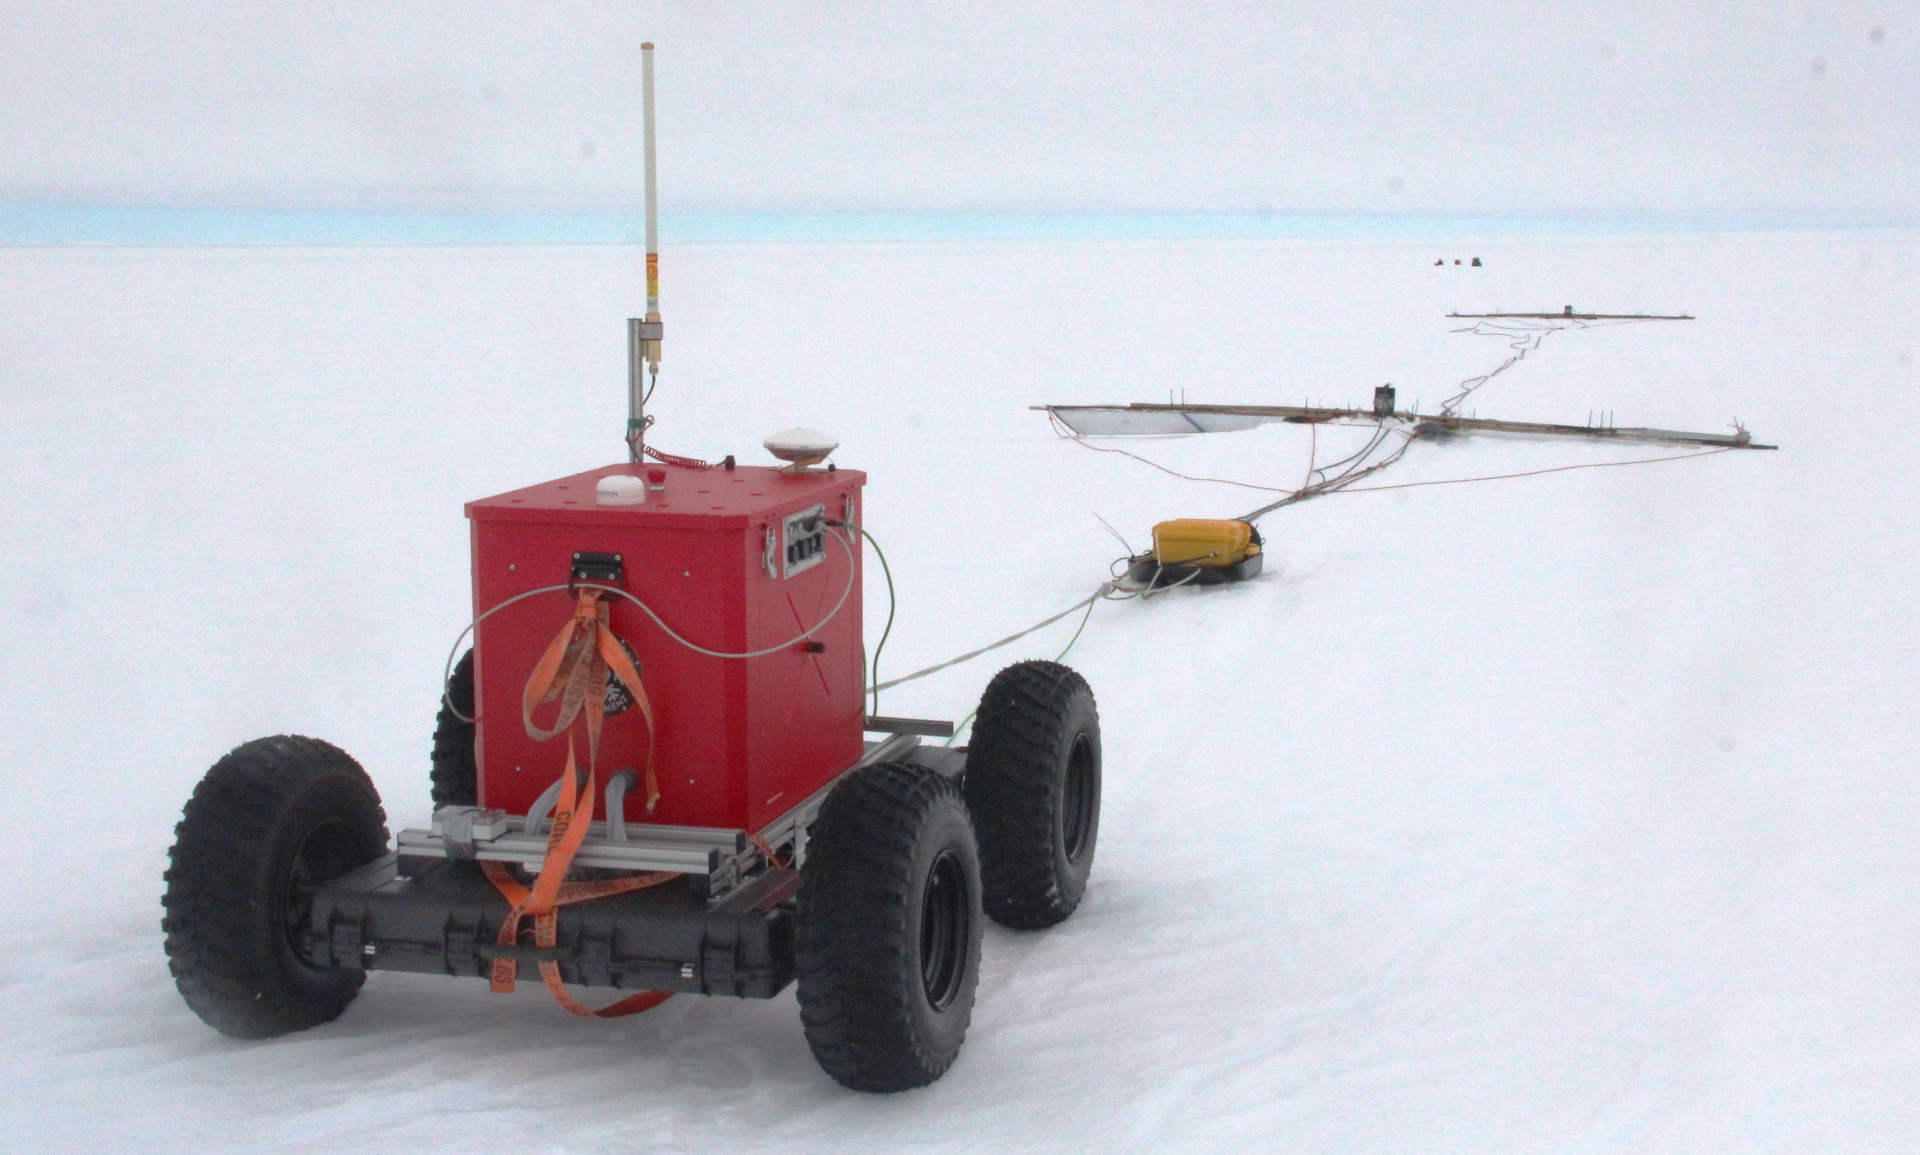
\includegraphics[width=0.8\textwidth]{Figures/ApRES/Rover/HF/hf-apres-subzero.jpg}
    };
    \begin{scope}[x={(img.south east)}, y={(img.north west)}]
      
      % Temporary grid
      % \draw[gray,step=0.1] (img.south west) grid (img.north east);
      % End temporary grid

      \contourlength{1pt}
      \node[anchor=east] at (0.33, 0.8) {\contour{white}{ UHF control radio}};
      \node[anchor=east] at (0.31, 0.6) {\contour{white}{Backup GPS}};
      \node[anchor=south] at (0.42, 0.63) {\contour{white}{RTK-GPS}};
      \node[anchor=west] at (0.87, 0.73) {\contour{white}{Tx}};
      \node[anchor=west] at (0.92, 0.62) {\contour{white}{Rx}};
      \node[anchor=west] at (0.65, 0.52) {\contour{white}{HF ApRES}};
      \node[anchor=south] at (0.24, 0.29) {\contour{white}{IMU}};
      \node[anchor=south] at (0.82, 0.73) {\contour{white}{IMU}};
      \node[anchor=south east] at (0.72,0.65) {\contour{white}{IMU}};

      % Draw distance labels
      \draw[latex-latex, line width=0.5pt, ucl_red] (0.81,0.72) -- 
        node[midway,above,anchor=south east,inner sep=1pt,ucl_red] {\contour{white}{40m}} (0.73,0.645);
      \draw[latex-latex, line width=0.5pt, ucl_red] (0.72,0.63) -- 
        node[midway,above,anchor=south east,inner sep=1pt,ucl_red] {\contour{white}{10m}} (0.652,0.552);
      \draw[latex-latex, line width=0.5pt, ucl_red] (0.6,0.5) --
        node[midway,above,ucl_red] {\contour{white}{10m}} (0.45,0.4);
      % \draw[ucl_red, line width=1pt] (0.76, 0.4) rectangle (0.83, 0.8);
      % \node[ucl_red, anchor=south] at (0.79, 0.8) {\contour{white}{\scriptsize 10dB Atten.}};

    \end{scope}
  \end{tikzpicture}
  \caption{
    SubZero rover and HF ApRES configuration used for start-stop and kinematic
    synthetic aperture radar acquisitions at groundling line.
  }
  \label{FigureHFApRESSubZeroConfiguration}
\end{figure}

\apresdoc
{2021-12-29\_215659.dat}
{Neumayer III,500m W of Station}
{\textbf{Antenna Orientation: Endfire, Neumayer}. No additional attenuations. Antennas rotated so they are aligned N-S and cables N-S.  Similar to above but with noise in upper layers. 14m separation.  Cables 'smooth' in line with antennas.  Reduced power code to 0.}
{2021-12-29 21:58:31.000}
{6,6,6,6}
{30,20,10,0}
{1.000}
{20}
{40}
{4}
{4}
{1}
{0}
{12.266}
{FigureHFApRESEndfireNeumayer}

\apresdoc{2021-12-29\_220442.dat}
{Neumayer III,500m W of Station}
{\textbf{Antenna Orientation: Broadside, Neumayer}. No additional attenuations. Antennas rotated so they are aligned E-W but Tx at N and Rx at S.  Similar to above but with noise in upper layers. 14m separation.  Cables 'smooth' in line with antennas.  Reduced power code to 0.}
{2021-12-29 22:04:45.000}
{6,6,6,6}
{30,20,10,0}
{1.000}
{20}
{40}
{4}
{4}
{1}
{0}
{12.258}
{FigureHFApRESBroadsideNeumayer}

\apresdoc{2022-01-05\_174254.dat}
{Grounding Line Camp}
{\textbf{Antenna Orientation: Endfire, Grounding Line}. Additional attenuator 10dB Rx, 0dB Tx.  Cable length Tx 25m, Rx 25m and separate antennas to maximum length (30m).  Antennas return to endfire.  Clipping across all AF settings.  No clear basal return.}
{2022-01-05 17:43:31.000}
{-14,-4,6}
{0,0,0}
{1.000}
{20}
{40}
{3}
{120}
{40}
{127}
{12.238}
{FigureHFApRESEndfireGroundingLine}

\apresdoc{2022-01-05\_171029.dat}
{Grounding Line Camp}
{\textbf{Antenna Orientation: Broadside, Grounding Line}. Additional attenuator 10dB Rx, 0dB Tx.  Increase Tx cable to 25m (Rx 5m) and separate antennas to maximum length (30m).  Antennas rotated broadside.  Bed clearer (higher SNR)? Some clipping in signal.  Repeated as before - ringing reduced?}
{2022-01-05 17:10:51.000}
{-14,-4,6}
{0,0,0}
{1.000}
{20}
{40}
{3}
{120}
{40}
{127}
{12.238}
{FigureHFApRESBroadsideGroundingLine}

\subsection{Synthetic Aperture Radar Measurements}
The test site chosen for the HF ApRES SAR measurements was selected to coincide
with the series of basal terraces observed in the PulseEKKO data located in the
finely gridded region of Figure \ref{fig:overview}.  The HF ApRES system was
towed into position on 7\textsuperscript{th} January, configured according to
\ref{FigureHFApRESSubZeroConfiguration} and initial testing was conducted,
including the resolution of a software navigation issue with the rover.  Two
modes of measurement were conducted with the HF ApRES: a start-stop profile
where the instrument was repositioned in steps of \SI{1}{\metre} increments
along the desired profile direct, and kinematic profiles where the radar was set
to continuously measure while towed along the profile by the SubZero rover at
speeds of approximately \SI{0.7}{\metre\per\second} to
\SI{1}{\metre\per\second}.  For all measurement modes, the radar was configured
with the parameters listed in Table \ref{TableHFApRESMeasurementParams}.

\begin{table}[h]
  \rowcolors{2}{gray!25}{white}
  \centering\begin{tabular}{l c r l}
    \hline
    \rowcolor{gray!50}
    Parameter & Symbol & \multicolumn{2}{c}{Value} \\
    \hline
    Centre Frequency & $f_c$ & 30 & \si{\mega\hertz} \\
    Bandwidth & $B$ & 20 & \si{\mega\hertz} \\
    Pulse Duration & $T$ & 1 & \si{\second} \\
    Transmit Power & $P_T$ & 0.1 & \si{\watt} \\
    AF Gain & $G_{AF}$ & 6 & \si{\deci\bel} \\
    RF Attenuation & $A_{RF}$ & 10 & \si{\deci\bel} \\
    RF Atten. (External) & $A_{RFExt}$ & 10 &  \si{\deci\bel} \\
    Antenna Separation & $S_{Ant}$ & 40 & \si{\metre} \\
    Rover Separation & $S_{Rov}$ & 10 & \si{\metre} \\
    \hline
    
  \end{tabular}
  \caption{Radar configuration parameters common to both the start-stop and
  kinematic the HF ApRES SAR measurements}
  \label{TableHFApRESMeasurementParams}
\end{table}

\subsubsection{Start-Stop Measurement}

On the 7\textsuperscript{th} January, \SI{192}{\metre} of the intended profile covered .  The rover was left in position overnight and the
profile was resumed to cover the remaining \SI{710}{\metre} over approximately 5
hours, including one hour of downtime.  For

  
\begin{figure}[h]
  \centering 
  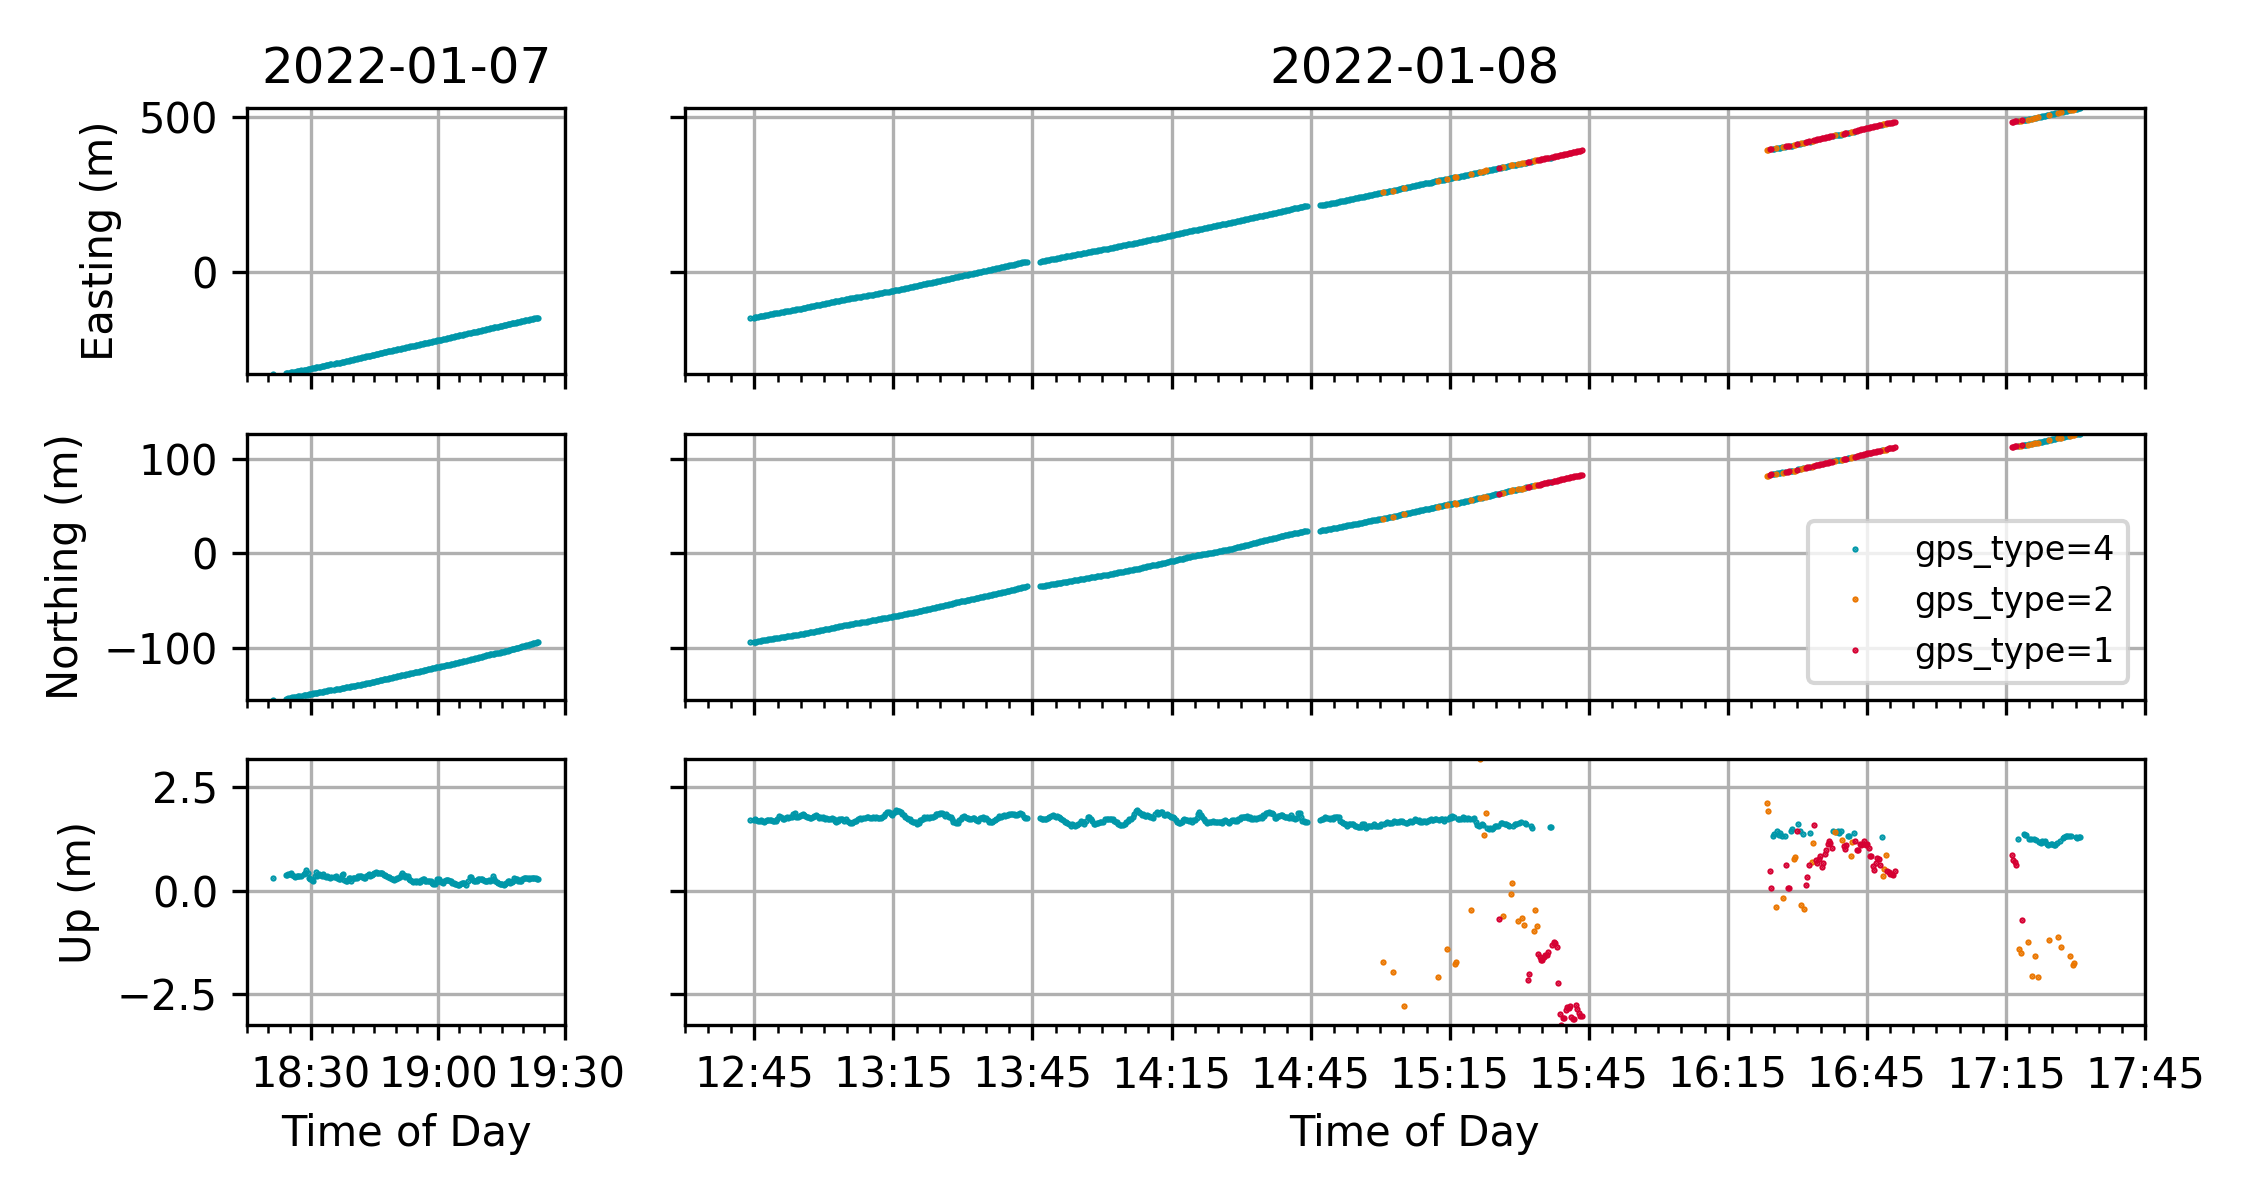
\includegraphics{../../Doc/ApRES/Rover/HF/StartStop/StartStopRawPositions.png}
  \caption{Recorded GPS positions for rover during start-stop acquisitions on
  7\textsuperscript{th} and 8\textsuperscript{th} of January, 2022.  A
  \texttt{gps\_type} value of 4 indicates RTK positioning, while values of 2 and
  1 indicate reduced accuracy GPS fixes.}
  \label{<label>}
\end{figure}

\pagebreak
\section{cApRES: Data example, field picture, system setup and site specifics}
\label{SeccApRES}
\textbf{RE,JH}


\pagebreak
\section{Rover-ApRES: Data example, field picture, system setup and site specifics}
\label{SecRoverApRES}
\textbf{RE}

%\ProtocolTable{Setup PulseEkko Radar}{N/A}{PulseEkko 50 MHz}{N/A}{I. Koch}{N/A}

% \begin{minipage}[t]{\textwidth}
%
% \end{minipage}



\end{document}